\subsection{Modelagem}

O eProfile é um sistema orientado a agentes, onde a metodologia utilizada para a modelagem é a Prometheus\cite{prometheus}. Esta metodologia define um processo detalhado para a especificação, projeto, implementação e teste/depuração de sistemas de software orientados a agentes.\cite{prometheus-book}

\begin{figure}
  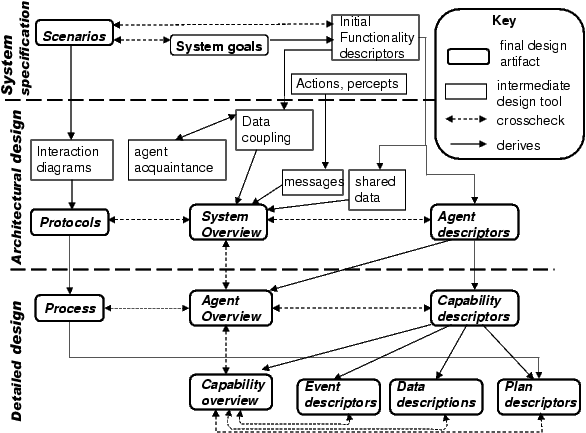
\includegraphics[width=0.5\textwidth]{imagens/prometheus.png}
  \caption{Processo de projeto segundo a metodologia Prometheus \cite{prometheus-book}}
  \label{fig:metodologia}
\end{figure}

A metodologia Prometheus, ilustrada na Figura~\ref{fig:metodologia} define que o primeiro passo da modelagem de um sistema é a identificação dos objetivos inciais do sistema. De acordo com o modelo do eProfile, os objetivos do sistema são:

\begin{itemize}
  \item Gerenciar múltiplos perfis;
  \item Comunicar-se com um (ou mais) gerenciadores de trilhas;
  \item Receber as regras de processamento dos clientes;
  \item Inferir dados de perfil através da análise das trilhas, de acordo com as regras definidas pelos clientes;
  \item Aceitar requisições de informações de perfil pelos clientes.
\end{itemize}


